%!TEX root = main.tex

\section*{Introduction}

In just a few years, next-generation sequencing (NGS) technologies have revolutionized the study of evolution and ecology in both model and non-model organisms, and have become established as standard tools in molecular ecology.

Not really what we will say here.

Don't forget to talk about Anthony Almudevar's visionary method for GSI power assessement \citep{almudevar2000exact}


\section*{Methods}

Something here.

\subsection*{Genomic Simulation Pedigrees}

For the purposes here, we define blah, blah.

\subsection*{Another subsection}



\subsection*{And a third}

Blah, blah blobbity blah.


\begin{figure*}
\begin{center}
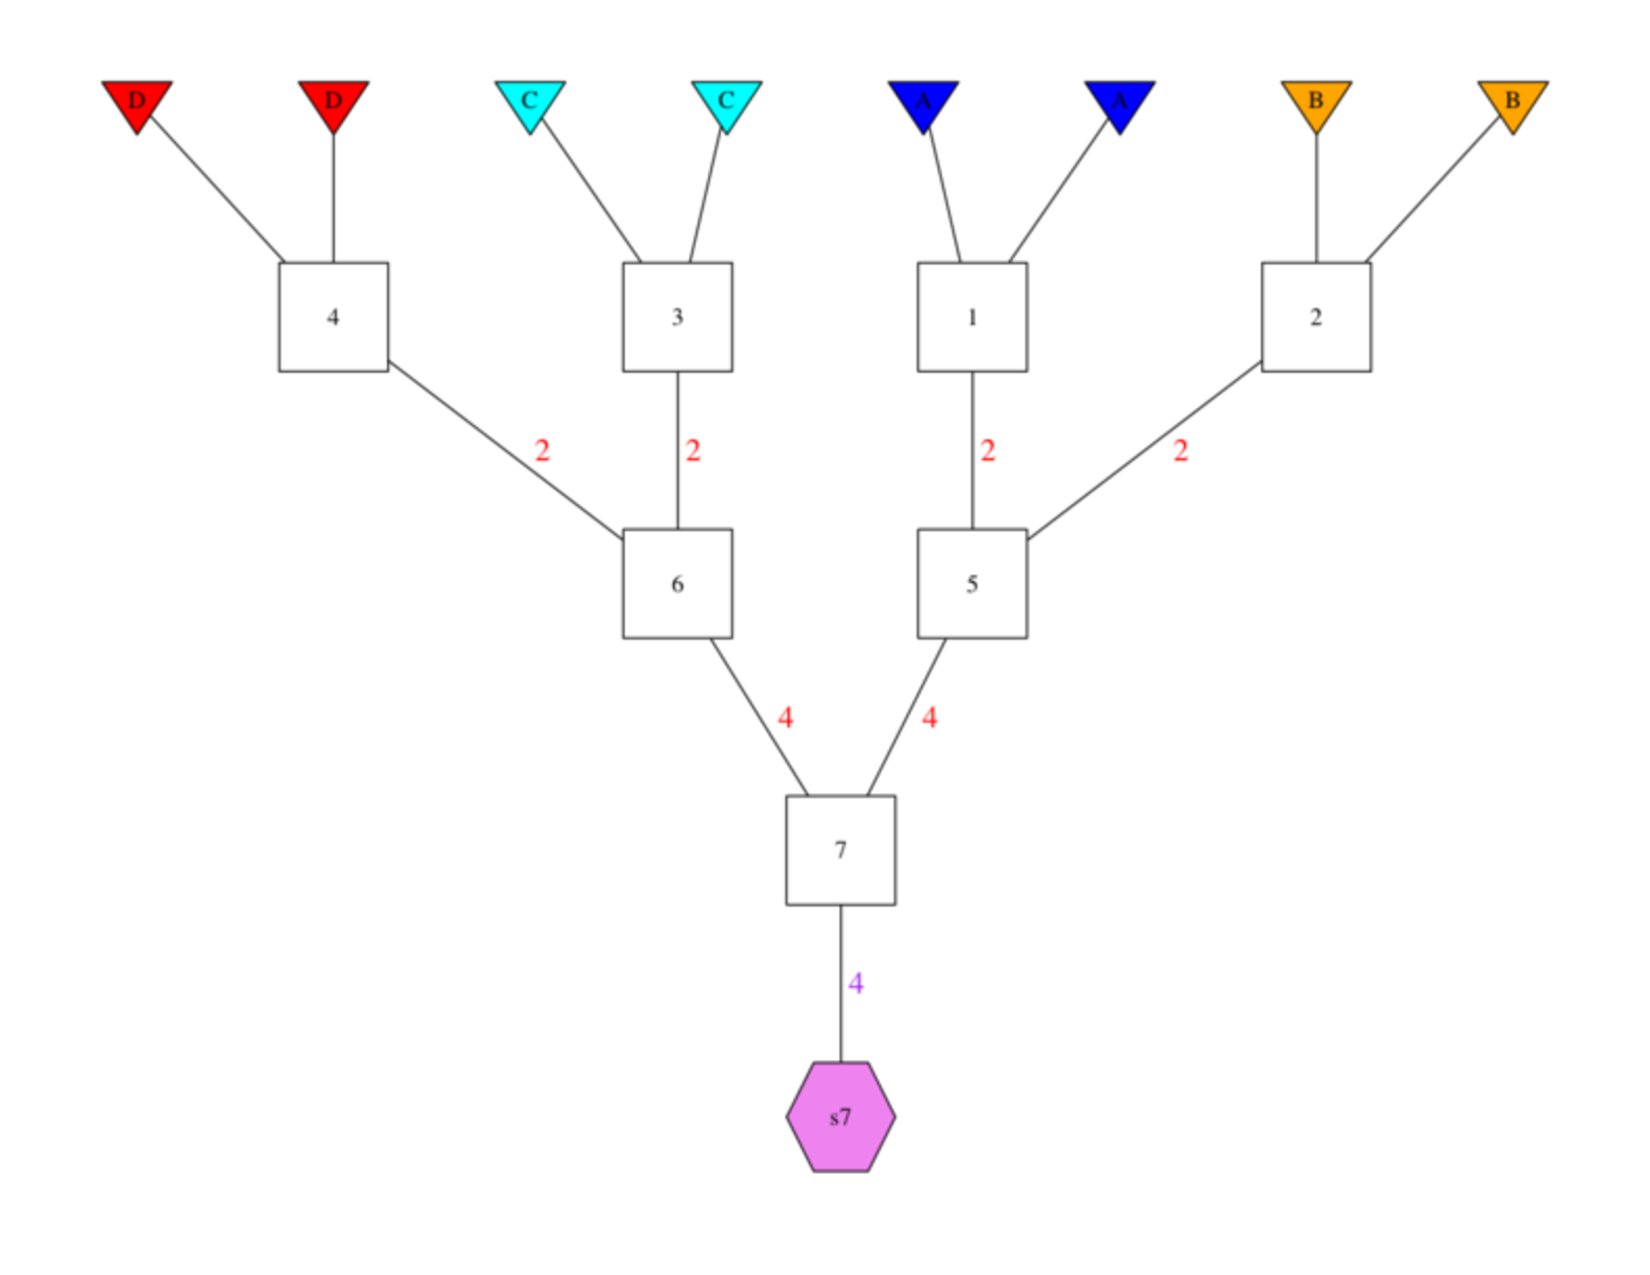
\includegraphics[width=0.8\textwidth]{images/gsp4-700.pdf}
\end{center}
\caption[]{Stick this thing in somewhere}
\end{figure*}


Not visible in the static plots are a number of dynamic features in the Shiny app display.
Values of filtering criteria for a single locus can be changed in real time in the app, and the results are updated in the adjacent genotype biplot.
Furthermore, it is possible to highlight points (representing individual samples) in the plot for one locus, and then observe the placement of those same selected samples at other loci.
This is particularly well-suited to identifying samples with aberrant genotypes across multiple loci---a good indicator of contamination or other issues with the sample.  

\section*{Discussion}
Hey! Let's discuss this!



\section*{Acknowledgements}
We thank the members of the Molecular Ecology and Genetic Analysis (MEGA) team at NOAA SWFSC's Fisheries Ecology Division, etc. etc. .